Next, we focus on the MISO case and investigate the influence of transmit antenna $M$ and subband $N$ on the R-E performance over typical multipath FF and FS channels. Thanks to the decoupling approach, the predetermined beamforming phases ${\mathbf{\Phi }}_I^ \star ,{\mathbf{\Phi }}_P^ \star $ are optimal for MISO and the computational complexity is irrelevant to $M$. Fig. \ref{fig:miso-channel} shows the frequency response employed in the optimization for $M = 2$ and 3.

\begin{figure}[ht]
  \centering
  \subfigure[$M = 2$]{
    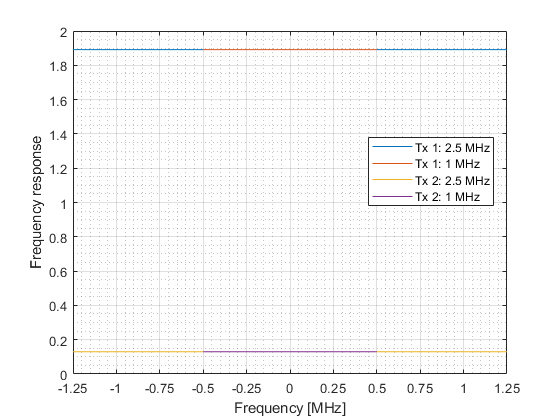
\includegraphics[width=0.48\textwidth]{miso_frequency_flat_channel_2tx}\label{fig:miso-frequency-flat-channel-2tx}}
  \subfigure[$M = 3$]{
    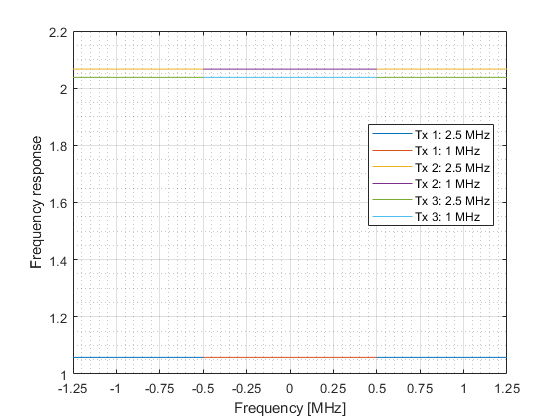
\includegraphics[width=0.48\textwidth]{miso_frequency_flat_channel_3tx}\label{fig:miso-frequency-flat-channel-3tx}}
  \caption{Frequency response of the MISO FF channels}
  \label{fig:miso-channel}
\end{figure}

The corresponding R-E regions for $N = 4$ and 8 are illustrated in Fig. \ref{fig:miso-re}.

\begin{figure}[ht]
  \centering
  \subfigure[$N = 4$]{
    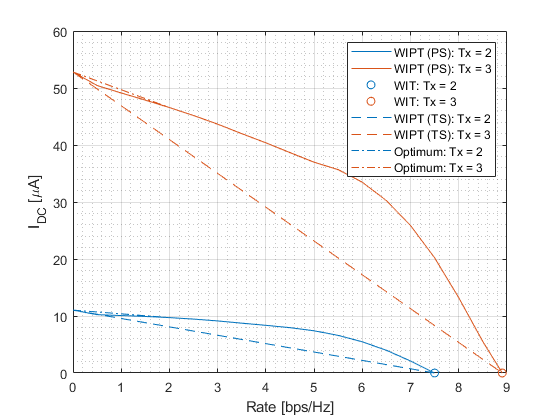
\includegraphics[width=0.48\textwidth]{miso_re_subband_4}\label{fig:miso-re-subband-4}}
  \subfigure[$N = 8$]{
    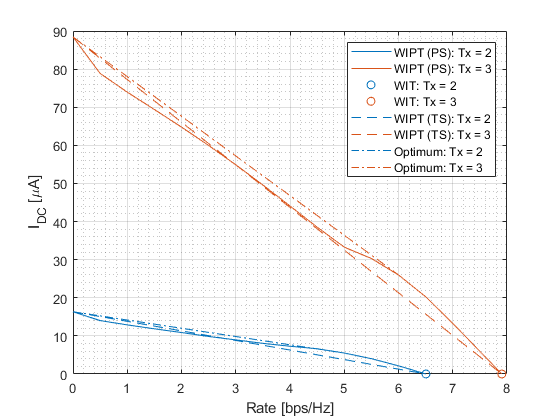
\includegraphics[width=0.48\textwidth]{miso_re_subband_8}\label{fig:miso-re-subband-8}}
  \caption{R-E region vs $M$ and $N$ over typical FF channels}
  \label{fig:miso-re}
\end{figure}

A first observation is that the concavity-convexity start to appear from $N = 4$ for the MISO systems, in contrast to $N = 8$ in the previous SISO case. The trend becomes more obvious as $N$ increases. The plots also suggest that a large $M$ can significantly boost the energy benefit of the multisine waveform. In this particular instance, raising $M$ from 2 to 3 produce a current gain of around 400 \%. Although this value partially results from the difference in channel amplitude, it highlights the benefit of using multiple antennas in WIPT. The reason is that increasing $M$ essentially enhances the subchannels such that the terms contributing to the harvested current are amplified. Also, a smaller $N$ is needed to achieve a certain output current level, which further reduces the signal PAPR. Hence, increasing $M$ can be a possible solution for PAPR-constrained systems. Moreover, a combination of TS (between WPT and WIPT) at a low rate and PS at high rate guarantees the optimal R-E region as a convex hull.

To eliminate the influence of channel randomness, we investigate the rate and energy performance for 100 FF channels with $N = 4$. Fig. \ref{fig:miso-cdf} shows the Cumulative Distribution Function (CDF) of maximum rate and current that correspond to WIT and WPT respectively. It is less interesting for WIPT since the variation trend of the R-E tradeoff is not presented. A better representation is required to avoid channel randomness and characterize the general R-E region.

\begin{figure}[ht]
  \centering
  \subfigure[Rate]{
    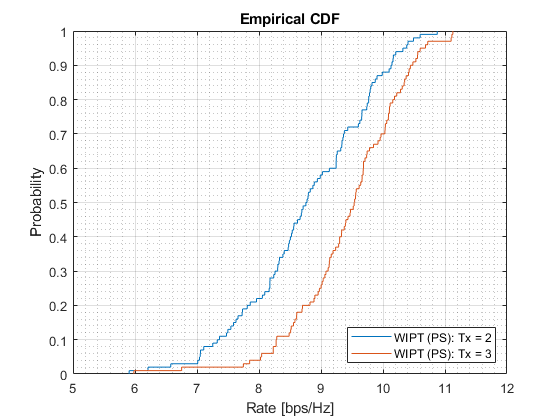
\includegraphics[width=0.48\textwidth]{miso_cdf_rate}\label{fig:miso-cdf-rate}}
  \subfigure[Current]{
    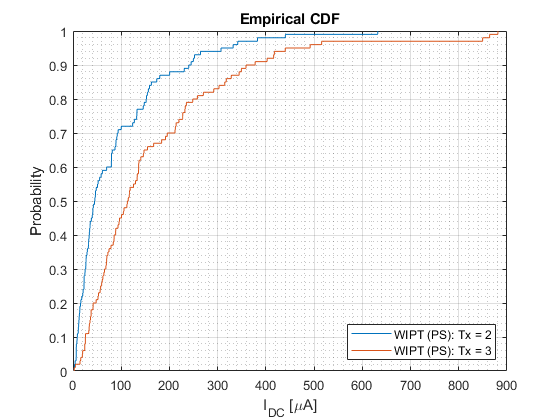
\includegraphics[width=0.48\textwidth]{miso_cdf_current}\label{fig:miso-cdf-current}}
  \caption{Rate and current CDF vs $M$ for MISO FF channels}
  \label{fig:miso-cdf}
\end{figure} 